% 5. Results (transferred from docs/paper/paper_draft.md)
\section{Results}
\label{sec:05_results}

\textbf{Run completion.} All 155 runs across the three experiments completed and passed the technical gate (30 + 25 + 100).

\textbf{Phase 8 (EB graph, fixed split).} Drosophila w20 minus rewired patient ROC AUC was −0.015 ± 0.041 (Drosophila higher in 2 of 5 seeds). On ROC AUC, EB Drosophila had the lowest mean of the graph models (0.927 ± 0.044, against 0.933–0.963 for the controls). All graph models exceeded the CNN baseline (0.900 ± 0.009).

\textbf{Phase 9 (visual graph, fixed split).}

\begin{itemize}
\item \textbf{Patient ROC AUC:} Visual Drosophila 0.944 ± 0.029, rewired 0.927 ± 0.053, ER 0.931 ± 0.037, WS 0.960 ± 0.025, BA 0.927 ± 0.044.
\item \textbf{Paired difference:} Drosophila − rewired was +0.017 ± 0.061 (higher in 3 of 5 seeds). This was small relative to seed-to-seed variability on a 21-patient test split.
\end{itemize}

\begin{table*}[!t]
\settablenumber{S1}
\centering
\footnotesize
\caption{Earlier fixed-split experiments (patient ROC AUC, test = 21 patients, 5 seeds). † Phase 8 CNN reference, not retrained.}
\label{tab:S1}
\begin{tabular}{lccccccc}
\toprule
\textbf{Experiment} & \textbf{Drosophila} & \textbf{Rewired} & \textbf{ER} & \textbf{WS} & \textbf{BA} & \textbf{CNN} & \textbf{Drosophila − rewired} \\
\midrule
Phase 8, EB w20 & 0.927 ± 0.044 & 0.942 ± 0.041 & 0.960 ± 0.018 & 0.933 ± 0.039 & 0.963 ± 0.036 & 0.900 ± 0.009 & −0.015 ± 0.041 \\
Phase 9, visual (w≥1) & 0.944 ± 0.029 & 0.927 ± 0.053 & 0.931 ± 0.037 & 0.960 ± 0.025 & 0.927 ± 0.044 & 0.900 ± 0.009 † & +0.017 ± 0.061 \\
\bottomrule
\end{tabular}
\end{table*}

\textbf{Phase 10 (leakage-safe CV, main result).}

\begin{itemize}
\item \textbf{Pooled OOF patient ROC AUC (Table III):} CNN 0.834 ± 0.028, Visual Drosophila 0.864 ± 0.033, rewired 0.874 ± 0.054, WS 0.874 ± 0.025.
\item \textbf{Fold-level patient ROC AUC (Table IV):} CNN 0.865 ± 0.041, Drosophila 0.925 ± 0.027, rewired 0.926 ± 0.029, WS 0.934 ± 0.030.
\item \textbf{Primary comparison (Table V, Fig. 5):} across 25 paired fold×seed runs, Drosophila − rewired patient ROC AUC was \textbf{−0.002 ± 0.030} (12 higher, 13 lower, 0 tied). The fold-level paired difference was \textbf{−0.002 ± 0.008}, with fold means of −0.001, −0.001, +0.004, −0.015 and +0.005. Slice-level ROC AUC gave −0.004 ± 0.021 (8 higher / 17 lower); patient balanced accuracy gave −0.016 ± 0.171.
\item \textbf{Secondary topology comparison:} Drosophila − WS was −0.009 ± 0.040, with a negative fold-level mean in all five folds (fold-level −0.009 ± 0.005).
\item \textbf{Architectural comparison:} Drosophila − CNN was +0.060 ± 0.063 (24 of 25 pairs positive). Because the models differ in architecture and parameter count, this is not a topology comparison.
\end{itemize}

\begin{table*}[!t]
\settablenumber{III}
\centering
\footnotesize
\caption{Phase 10 pooled out-of-fold patient-level performance (mean ± SD across 5 seeds; threshold 0.5; each seed's OOF set contains all 171 patients exactly once).}
\label{tab:III}
\begin{tabular}{lccccccc}
\toprule
\textbf{Model} & \textbf{Params} & \textbf{ROC AUC} & \textbf{Balanced acc.} & \textbf{Sensitivity} & \textbf{Specificity} & \textbf{F1} & \textbf{Precision} \\
\midrule
CNN baseline & 41,921 & 0.834 ± 0.028 & 0.766 ± 0.033 & 0.791 ± 0.036 & 0.741 ± 0.067 & 0.780 ± 0.026 & 0.771 ± 0.044 \\
Visual Drosophila & 44,411 & 0.864 ± 0.033 & 0.733 ± 0.055 & 0.879 ± 0.045 & 0.588 ± 0.075 & 0.778 ± 0.044 & 0.699 ± 0.047 \\
Visual rewired & 44,411 & 0.874 ± 0.054 & 0.749 ± 0.066 & 0.870 ± 0.106 & 0.629 ± 0.156 & 0.786 ± 0.055 & 0.727 ± 0.085 \\
Visual WS & 44,411 & 0.874 ± 0.025 & 0.762 ± 0.060 & 0.872 ± 0.058 & 0.651 ± 0.174 & 0.797 ± 0.028 & 0.743 ± 0.083 \\
\bottomrule
\end{tabular}
\end{table*}

\begin{table*}[!t]
\settablenumber{IV}
\centering
\footnotesize
\caption{Phase 10 fold-level patient ROC AUC (mean over the 5 seeds within each outer fold).}
\label{tab:IV}
\begin{tabular}{lccccccc}
\toprule
\textbf{Model} & \textbf{Fold 1} & \textbf{Fold 2} & \textbf{Fold 3} & \textbf{Fold 4} & \textbf{Fold 5} & \textbf{Mean ± SD} & \textbf{Median [min, max]} \\
\midrule
CNN baseline & 0.905 & 0.862 & 0.899 & 0.856 & 0.803 & 0.865 ± 0.041 & 0.862 [0.803, 0.905] \\
Visual Drosophila & 0.938 & 0.881 & 0.919 & 0.936 & 0.951 & 0.925 ± 0.027 & 0.936 [0.881, 0.951] \\
Visual rewired & 0.939 & 0.881 & 0.915 & 0.951 & 0.946 & 0.926 ± 0.029 & 0.939 [0.881, 0.951] \\
Visual WS & 0.944 & 0.883 & 0.931 & 0.951 & 0.958 & 0.934 ± 0.030 & 0.944 [0.883, 0.958] \\
\bottomrule
\end{tabular}
\end{table*}

\begin{table*}[!t]
\settablenumber{V}
\centering
\footnotesize
\caption{Primary paired topology comparison: Visual Drosophila − Visual rewired (Phase 10).}
\label{tab:V}
\begin{tabular}{lccc}
\toprule
\textbf{Metric} & \textbf{All 25 fold×seed pairs} & \textbf{Higher / lower / tied} & \textbf{Fold-level (5 values)} \\
\midrule
Patient ROC AUC & −0.002 ± 0.030 & 12 / 13 / 0 & −0.002 ± 0.008 \\
Slice ROC AUC & −0.004 ± 0.021 & 8 / 17 / 0 & −0.004 ± 0.013 \\
Patient balanced accuracy & −0.016 ± 0.171 & 10 / 15 / 0 & −0.016 ± 0.029 \\
\bottomrule
\end{tabular}
\end{table*}

\begin{figure*}[!t]
\centering
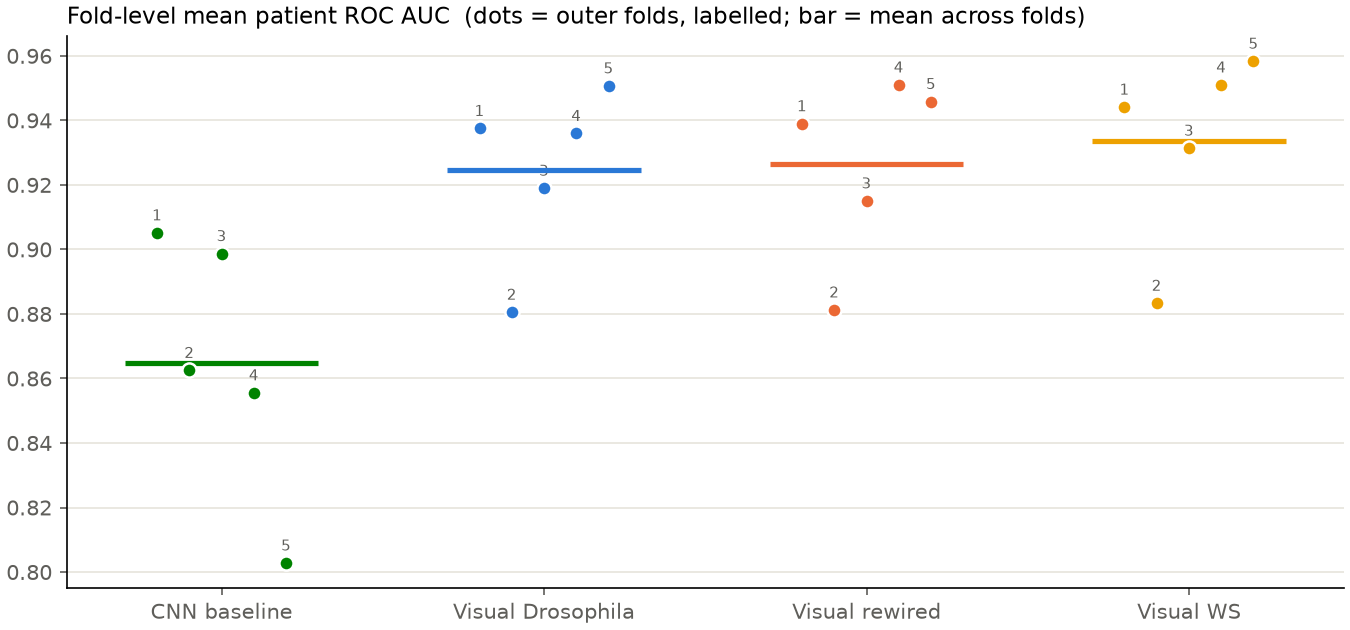
\includegraphics[width=\textwidth]{figures/fig2_fold_level_patient_auc.png}
\caption{Phase 10 fold-level patient ROC AUC. Dots are the five outer-fold means (seeds averaged within each fold, labelled with the fold number); bars are the means across folds. Frozen figure: \texttt{docs/results/phase10/fig2\_fold\_level\_patient\_auc.png}.}
\label{fig:fig2_fold_level_patient_auc}
\end{figure*}

\begin{figure*}[!t]
\centering
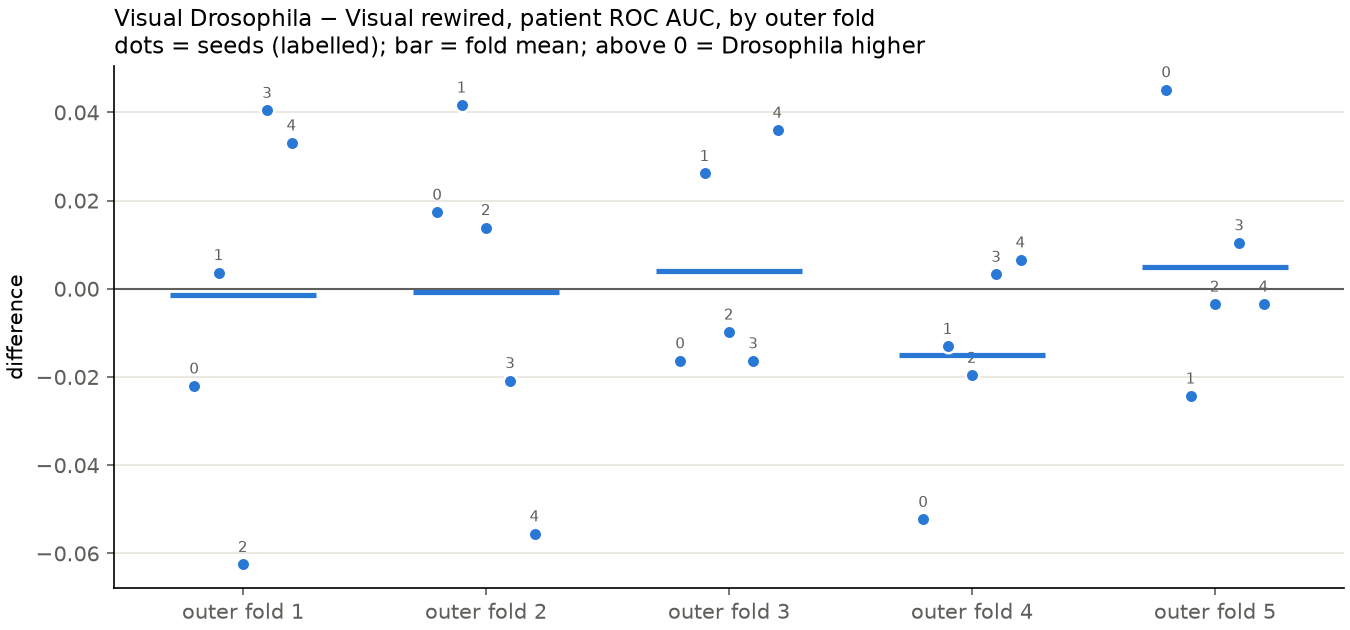
\includegraphics[width=\textwidth]{figures/fig4_paired_drosophila_rewired_by_fold.png}
\caption{Primary paired comparison, Visual Drosophila − Visual rewired patient ROC AUC, per outer fold. Dots are seeds (labelled), bars are fold means, and values above 0 mean Drosophila was higher. Frozen figure: \texttt{docs/results/phase10/fig4\_paired\_drosophila\_rewired\_by\_fold.png}.}
\label{fig:fig4_paired_drosophila_rewired_by_fold}
\end{figure*}

\begin{figure*}[!t]
\centering
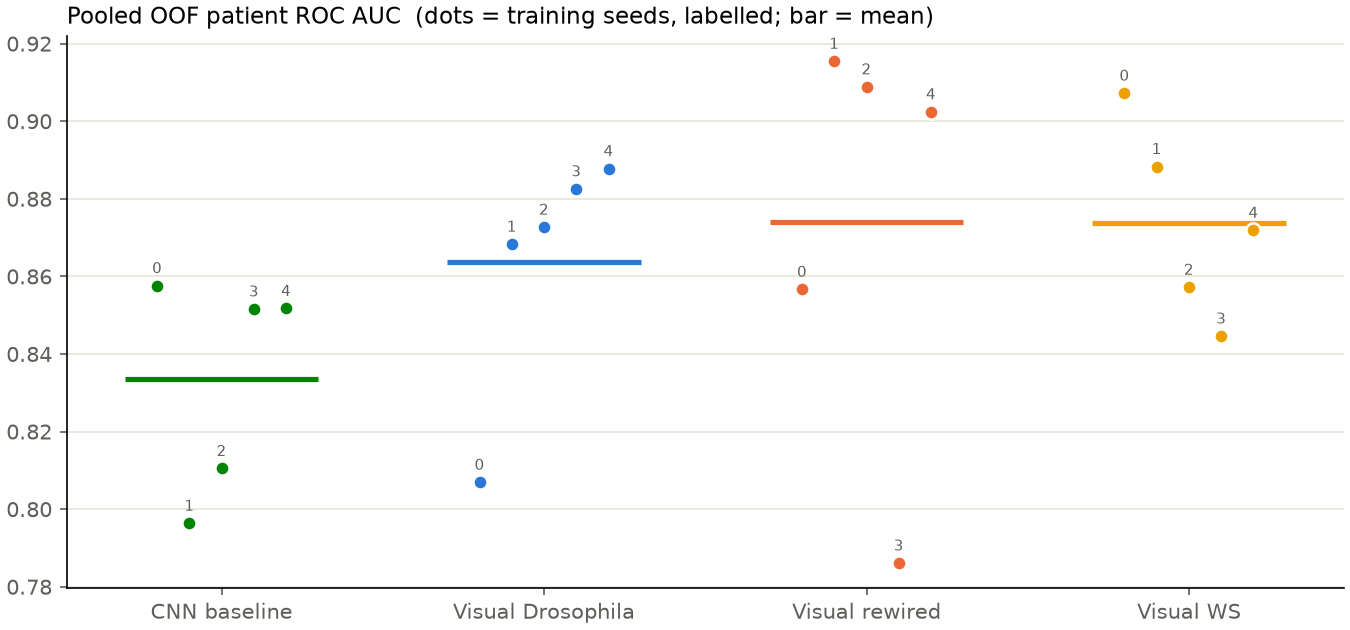
\includegraphics[width=\textwidth]{figures/fig3_oof_patient_auc.png}
\caption{Pooled out-of-fold patient ROC AUC per model; dots are training seeds (labelled), bars are means. Frozen figure: \texttt{docs/results/phase10/fig3\_oof\_patient\_auc.png}.}
\label{fig:fig3_oof_patient_auc}
\end{figure*}

\textbf{Threshold-dependent metrics.} At the frozen threshold of 0.5, the graph models had higher pooled OOF sensitivity (0.87–0.88) but lower specificity (Drosophila 0.588 ± 0.075, rewired 0.629 ± 0.156, WS 0.651 ± 0.174) than the CNN (sensitivity 0.791 ± 0.036, specificity 0.741 ± 0.067). As a result, pooled OOF balanced accuracy was comparable or higher for the CNN (0.766 ± 0.033) than for the graph models (0.733–0.762), despite its lower ROC AUC.

\begin{figure*}[!t]
\centering
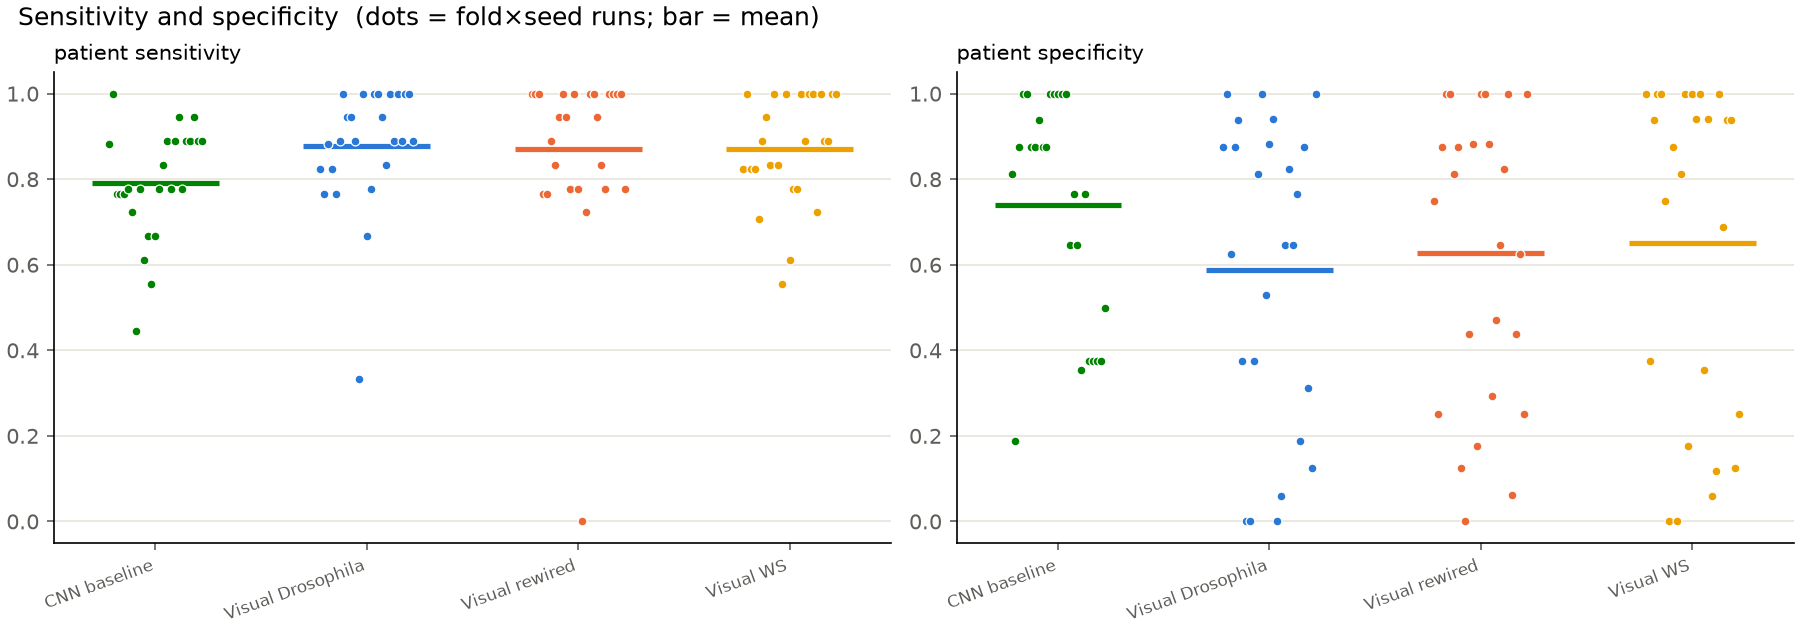
\includegraphics[width=\textwidth]{figures/fig7_sensitivity_specificity.png}
\caption{Patient-level sensitivity and specificity at the fixed 0.5 threshold across all 25 fold×seed runs per model (Phase 10). Frozen figure: \texttt{docs/results/phase10/fig7\_sensitivity\_specificity.png}.}
\label{fig:fig7_sensitivity_specificity}
\end{figure*}

\textbf{Pooled vs fold-level AUC.} Pooled OOF ROC AUC was consistently lower than fold-level ROC AUC (Drosophila 0.864 vs 0.925), because pooling mixes probability scales from five separately trained models.

\textbf{Runtime.} Training took 147–169 s per run on CPU; inference took about 2.1 ms per slice for all models.
